\chapter{Specifikacija programske potpore}
		
	\section{Funkcionalni zahtjevi}
			
			
			
			\noindent \textbf{Dionici:}
			
			\begin{packed_enum}
				
				\item Klijenti
				\item Iznajmljivači			
				\item Administratori sustava
				\item Razvojni tim 
				
			\end{packed_enum}
			
			\noindent \textbf{Aktori i njihovi funkcionalni zahtjevi:}
			
			
			\begin{packed_enum}
				\item  \underbar {Neregistrirani korisnik/posjetilac (inicijator) može:}
				
				\begin{packed_enum}
					
					\item pregledavati dostupne romobile
					\item odabrati romobil da dobije detaljnije podatke o njemu
					\item registrirati se u sustav, stvoriti novi korisnički račun
					
					
				\end{packed_enum}
			
				\item  \underbar{Klijent (inicijator) može:}
				
				\begin{packed_enum}
					\item pregledavati dostupne romobile
					\item pregledati osobne podatke na svome profilu i urediti ih 
					\item izbrisati svoj profil
					\item registrirati romobil
					\item iznajmiti romobil
					\item zamijeniti sliku romobila
					\item vratiti romobil
					\item pregledati svoje prethodne transakcije
					\item pogledati profil drugog korisnika
					\item pogledati razgovor s nekim drugim korisnikom
					\item poslati poruku drugom korisniku
					\item izbrisati razgovor s drugim korisnikom
					
				
					
				\end{packed_enum}
				\item  \underbar {Iznajmljivač (inicijator) može:}
				
				\begin{packed_enum}
				\item pogledati detaljne informacije o svom registriranom romobilu
				\item promijeniti informacije o registriranom romobilu
				\item izbrisati registrirani romobil
				\item postaviti oglas za registrirani romobil
				\item objaviti oglas za iznajmljivanje romobila na društvene mreže
				\item pregledati i uređivati svoj oglas
				\item izbrisati oglas za iznajmljivanje romobila
				\item prihvatiti ili odbiti zahtjev za iznajmljivanje
				\item poslati žalbu na zamjenu slika romobila 
				\item ocijeniti klijenta
				\item izbrisati svoju recenziju o drugom korisniku
				
			\end{packed_enum}
			\item  \underbar {Administrator (inicijator) može:}
			
			\begin{packed_enum}
		
			\item pregledati dostupne romobile i detalje o njima
			\item pregledati dokumentaciju za registraciju i prihvatiti ili odbiti zahtjev za registraciju
			\item pregledati svoj profil
			\item urediti svoj profil
			\item izbrisati svoj profil
			\item Izbrisati oglas
			\item odlučiti poništava li se zamjena slika ili ne
			\item pogledati profil drugog korisnika
			\item izbrisati recenziju o nekom korisniku
			\item blokirati korisnika
			\item odblokirati korisnika
			\item dodati drugom korisniku ulogu administratora
			\item oduzeti drugom administratoru ulogu administratora
			
			
		
			
			\end{packed_enum}
			\item  \underbar {Baza podataka(sudionik):}

			\begin{packed_enum}
				
				\item pohranjuje sve podatke o korisnicima i njihovim ovlastima
				
				\item pohranjuje sve podatke o romobilima, njihovim iznajmljivanjima i transakcijama
				
				
				
			\end{packed_enum}
			
			\item  \underbar {Banka (inicijator) može:}
			
			\begin{packed_enum}
				
			\item umanjiti iznos novca na računu klijenta za iznos cijene iznajmljivanja
			
			\item uplati cijenu iznajmljivanja iznajmljivaču na račun
			
			
			
			\end{packed_enum}
		\end{packed_enum}
			
			\eject 
			
			
				
			\subsection{Obrasci uporabe}
				
			
				
				\subsubsection{Opis obrazaca uporabe}
					
					
					\noindent \underbar{\textbf{UC1 - Pregledaj romobil}}
					\begin{packed_item}
	
						\item \textbf{Glavni sudionik: }Neregistrirani korisnik, klijent, administrator 
						\item  \textbf{Cilj:} Pregledati dostupne romobile i detalje o njima i ponudi
						\item  \textbf{Sudionici:} Baza podataka
						\item  \textbf{Preduvjet:} -
						\item  \textbf{Opis osnovnog tijeka:}
						
						\item[] \begin{packed_enum}
	
							\item Prilikom učitavanja aplikacije prikazuju se romobili dostupni za iznajmljivanje
							\item Korisnik pronalazi i odabire željeni romobil
							\item Korisniku se prikazuju detaljnije informacije o romobilu i uvjetima iznajmljivanja
						
						\end{packed_enum}
					\end{packed_item}
						
						\noindent \underbar{\textbf{UC2 - Registriraj se}}
						\begin{packed_item}
							
							\item \textbf{Glavni sudionik: } Neregistrirani korisnik
							\item  \textbf{Cilj:} Napraviti korisnički račun kojim se pristupa sustavu
							\item  \textbf{Sudionici:} Administrator, baza podataka
							\item  \textbf{Preduvjet:} -
							\item  \textbf{Opis osnovnog tijeka:}
							
							\item[] \begin{packed_enum}
								
								\item	Neregistrirani korisnik odabire opciju „Registriraj se“
								\item 	Neregistriranom korisniku prikazuje se stranica za registraciju
							    \item 	Neregistrirani korisnik unosi podatke za registraciju
								\item 	Unesena kopija osobne iskaznice i potvrda o nekažnjavanju šalju se administratoru na pregled
								\item 	Stvara se novi korisnički račun čiji se podatci pohranjuju u bazu podataka
								\item 	Neregistriranom korisniku se prikazuje stranica za čekanje odobrenja registracije
								
								 
								
							\end{packed_enum}
							
							\item  \textbf{Opis mogućih odstupanja:}
							
							\item[] \begin{packed_item}
								
								\item[3.a] Unos podataka u nedozvoljenom formatu ili unos već zauzetog nadimka ili e-mail adrese
								\item[] \begin{packed_enum}
									
									\item 	Neregistrirani korisnik dobiva odgovarajuću obavijest o neispravnosti podataka
									\item	Neregistrirani korisnik mijenja potrebne podatke i završava s unosom ili odustaje od registracije
									
									
								\end{packed_enum}
								
								
							\end{packed_item}
						\end{packed_item}
						\noindent \underbar{\textbf{UC3 - Odobri ili odbij registraciju}}
						\begin{packed_item}
							
							\item \textbf{Glavni sudionik: } Administrator
							\item  \textbf{Cilj: } Odlučiti o valjanosti kopije osobne iskaznice i potvrde o nekažnjavanju
							\item  \textbf{Sudionici: }Klijent, baza podataka
							\item  \textbf{Preduvjet: }Postoji barem jedan zahtjev za registraciju 
							\item  \textbf{Opis osnovnog tijeka:}
							
							\item[] \begin{packed_enum}
								
								\item Administrator pregledava dokumentaciju poslanu pri registraciji korisnika ili pri ponovnom slanju dokumentacije 
								\item Administrator odlučuje o potvrđivanju dokumenata i njegova odluka se zapisuje u bazu podataka
								\item Klijenta čija se registracija provjerava se preusmjerava na stranicu za prijavu
								
								
							\end{packed_enum}
						\end{packed_item}
						\noindent \underbar{\textbf{UC4 - Ponovno predaj dokumente}}
						\begin{packed_item}
							
							\item \textbf{Glavni sudionik: }Neregistrirani korisnik
							\item  \textbf{Cilj:} Ponovno predati kopiju osobne iskaznice i potvrdu o nekažnjavanju na pregled
							\item  \textbf{Sudionici:} Administrator, baza podataka
							\item  \textbf{Preduvjet:} Prethodno odbijen zahtjev za registraciju
							\item  \textbf{Opis osnovnog tijeka:}
							
							\item[] \begin{packed_enum}
								
								\item Neregistrirani korisnik unosi novu dokumentaciju za registraciju u sustav 
								\item Dokumentacija se šalje administratoru na pregled 
								\item Neregistriranom korisniku se prikazuje stranica za čekanje odobrenja registracije
								
								
							\end{packed_enum}
							
							\item  \textbf{Opis mogućih odstupanja:}
							
							\item[] \begin{packed_item}
								
								\item[1.a] Unos dokumentacije u nedozvoljenom formatu 
								\item[] \begin{packed_enum}
									
									\item Neregistrirani korisnik dobiva odgovarajuću obavijest o neispravnosti podataka  
									\item Neregistrirani korisnik ispravno unosi dokumentaciju i završava s unosom ili odustaje od ponovne predaje dokumentacije  
									
								\end{packed_enum}
								
								
							\end{packed_item}
						\end{packed_item}
						\noindent \underbar{\textbf{UC5 - Prijavi se}}
						\begin{packed_item}
							
							\item \textbf{Glavni sudionik: } Klijent, administrator
							\item  \textbf{Cilj:} Dobiti pristup određenim korisničkim funkcijama
							\item  \textbf{Sudionici:} Baza podataka
							\item  \textbf{Preduvjet:} Korisnik se registrirao i odobrena mu je registracija
							\item  \textbf{Opis osnovnog tijeka:}
							
							\item[] \begin{packed_enum}
								
								\item 	Korisnik odabire opciju „Prijavi se“
								\item 	Korisniku se prikazuje stranica za prijavu
								\item 	Korisnik unosi podatke za prijavu
								\item 	Prijava je odobrena i korisnik dobiva pristup svojim korisničkim funkcijama
								
								
								
								
							\end{packed_enum}
							
							\item  \textbf{Opis mogućih odstupanja:}
							
							\item[] \begin{packed_item}
								
								\item[3.a] Unos podataka koji ne odgovaraju nijednom registriranom korisniku u bazi podataka
								\item[] \begin{packed_enum}
									
									\item Korisnik dobiva odgovarajuću obavijest o neispravnosti podataka
									\item Korisnik mijenja potrebne podatke i završava s unosom ili odustaje od prijave
									
									
								\end{packed_enum}
								\item[4.a] Prijava nije odobrena jer korisnik čeka na odobrenje registracije
								\item[] \begin{packed_enum}
									
									\item Korisniku se prikazuje stranica za čekanje odluke o registraciji
								\end{packed_enum}
								\item[4.b] Prijava nije odobrena jer je korisniku odbijena dokumentacija za registraciju
								\item[] \begin{packed_enum}
									\item Korisnika se preusmjerava na stranicu za ponovnu predaju dokumentacije za registraciju
								\end{packed_enum}
								\item[4.c] Prijava nije odobrena jer je korisnik blokiran i nema pristup sustavu
								\item[] \begin{packed_enum}
									\item Korisnik dobiva obavijest da je blokiran i nema više pristup sustavu
								\end{packed_enum}
								
								
								
							\end{packed_item}
						\end{packed_item}
						\noindent \underbar{\textbf{UC6 - Odjavi se}}
						\begin{packed_item}
							
							\item \textbf{Glavni sudionik: } Klijent, administrator
							\item  \textbf{Cilj: } Odjaviti se iz sustava
							\item  \textbf{Sudionici: }Baza podataka
							\item  \textbf{Preduvjet: }Korisnik je prijavljen
							\item  \textbf{Opis osnovnog tijeka:}
							
							\item[] \begin{packed_enum}
								
								\item 	Korisnik odabire opciju „Odjavi se“
								\item 	Korisnik napušta sustav
								
								
							\end{packed_enum}
						\end{packed_item}
						\noindent \underbar{\textbf{UC7 - Pregledaj svoj profil}}
						\begin{packed_item}
							
							\item \textbf{Glavni sudionik: } Klijent, administrator
							\item  \textbf{Cilj:} Pregledati korisničke podatke svog profila
							\item  \textbf{Sudionici:} Baza podataka
							\item  \textbf{Preduvjet:} Korisnik je prijavljen
							\item  \textbf{Opis osnovnog tijeka:}
							
							\item[] \begin{packed_enum}
								
								\item Korisnik odabire opciju „Moj profil“ 
								\item Korisniku se prikazuje stranica vlastitog profila i svi njegovi korisnički podatci   
								\item Korisnik pregledava informacije o svom profilu 
							 
							\end{packed_enum}
						\end{packed_item}
						\noindent \underbar{\textbf{UC8 - Uredi svoj profil}}
						\begin{packed_item}
							
							\item \textbf{Glavni sudionik: }Klijent, administrator
							\item  \textbf{Cilj:}Promijeniti korisničke podatke i odlučiti koji će od njih biti javni, a koji privatni
							\item  \textbf{Sudionici:} Baza podataka
							\item  \textbf{Preduvjet:} Korisnik je prijavljen
							\item  \textbf{Opis osnovnog tijeka:}
							
							\item[] \begin{packed_enum}
								
								\item Korisnik na stranici svog profila odabire opciju „Uredi profil“
								\item Korisnik mijenja svoje korisničke podatke i njihovu dostupnost
								\item Korisnik potvrđuje promjene odabirom opcije „Spremi promjene“ 
								\item Baza podataka se ažurira 
								
								
							\end{packed_enum}
							
							\item  \textbf{Opis mogućih odstupanja:}
							
							\item[] \begin{packed_item}
								
								\item[2.a] Unos podataka u nedozvoljenom formatu ili unos već zauzetog nadimka ili e-mail adrese 
								\item[] \begin{packed_enum}
									
									\item Korisnik dobiva odgovarajuću obavijest o neispravnosti podataka 
									\item Korisnik mijenja potrebne podatke i završava s unosom ili odustaje od promjene 
									
								\end{packed_enum}
								\item[3.a] Korisnik ne potvrdi promjenu odabirom opcije „Spremi promjene“    
								\item[] \begin{packed_enum}
									
									\item Korisnik dobiva obavijest da nije spremio podatke prije izlaska iz prozora za promjenu podataka   
									\item Korisnik sprema promjene 
									
								\end{packed_enum}
								
								
								
							\end{packed_item}
						\end{packed_item}
						\noindent \underbar{\textbf{UC9 - Izbriši svoj profil}}
						\begin{packed_item}
							
							\item \textbf{Glavni sudionik: }Klijent, administrator
							\item  \textbf{Cilj:} Izbrisati svoj korisnički račun iz baze podataka
							\item  \textbf{Sudionici:} Baza podataka
							\item  \textbf{Preduvjet:} Korisnik je prijavljen
							\item  \textbf{Opis osnovnog tijeka:}
							
							\item[] \begin{packed_enum}
								
								\item Korisnik odabire opciju „Izbriši profil“
								\item Korisnik potvrđuje svoj odabir
								\item Korisnikov profil se briše iz baze podataka
								\item Otvara se stranica za registraciju
								
							\end{packed_enum}
							
						\end{packed_item}
						
						\noindent \underbar{\textbf{UC10 - Registriraj romobil}}
						\begin{packed_item}
							
							\item \textbf{Glavni sudionik: }Klijent
							\item  \textbf{Cilj: }Dodavanje romobila na popis svojih romobila
							\item  \textbf{Sudionici: }Baza podataka
							\item  \textbf{Preduvjet: }Klijent je prijavljen
							\item  \textbf{Opis osnovnog tijeka:}
							
							\item[] \begin{packed_enum}
								
								\item Klijent odabire opciju „Registriraj romobil“ 
								\item Klijent unosi podatke o romobilu i sliku trenutnog stanja romobila 
								\item Registracija romobila se zabilježi u bazi podataka 
								  
							\end{packed_enum}
							
							\item  \textbf{Opis mogućih odstupanja:}
							
							\item[] \begin{packed_item}
								
								\item[2.a] Unos podataka o romobilu u nedozvoljenom formatu 
								\item[] \begin{packed_enum}
									
									\item Korisnik dobiva odgovarajuću obavijest o neispravnosti podataka 
									\item Korisnik mijenja potrebne podatke i završava s unosom ili odustaje od registracije romobila 
									
								\end{packed_enum}
								
								
							\end{packed_item}
						\end{packed_item}
						\noindent \underbar{\textbf{UC11 - Pregledaj svoj romobil}}
						\begin{packed_item}
							
							\item \textbf{Glavni sudionik: }Iznajmljivač
							\item  \textbf{Cilj: }Pregledati detaljne informacije o svom registriranom romobilu
							\item  \textbf{Sudionici: }Baza podataka
							\item  \textbf{Preduvjet: }Iznajmljivač je prijavljen, ima barem jedan registrirani romobil
							\item  \textbf{Opis osnovnog tijeka:}
							
							\item[] \begin{packed_enum}
								
								\item Prikazuje se stranica s iznajmljivačevim registriranim romobilima
								\item Iznajmljivač pronalazi i odabire željeni romobil
								\item Iznajmljivaču se prikazuju detaljnije informacije o romobilu
							
							\end{packed_enum}
						\end{packed_item}
						\noindent \underbar{\textbf{UC12 - Uredi svoj romobil}}
						\begin{packed_item}
							
							\item \textbf{Glavni sudionik: }Iznajmljivač
							\item  \textbf{Cilj: }Promijeniti informacije o svom registriranom romobilu
							\item  \textbf{Sudionici:} Baza podataka
							\item  \textbf{Preduvjet:} Iznajmljivač je prijavljen, ima barem jedan registrirani romobil
							\item  \textbf{Opis osnovnog tijeka:}
							
							\item[] \begin{packed_enum}
								
								\item Prikazuje se stranica s iznajmljivačevim registriranim romobilima
								\item Iznajmljivač pronalazi i odabire željeni romobil i opciju „Uredi“
								\item Iznajmljivač mijenja informacije o romobilu
								\item Iznajmljivač potvrđuje promjene odabirom opcije „Spremi promjene“
								\item Baza podataka se ažurira
								
							\end{packed_enum}
							
							\item  \textbf{Opis mogućih odstupanja:}
							
							\item[] \begin{packed_item}
								
								\item[3.a] Unos podataka o romobilu u nedozvoljenom formatu
								\item[] \begin{packed_enum}
									
									\item Iznajmljivač dobiva odgovarajuću obavijest o neispravnosti podataka 
									\item Iznajmljivač mijenja potrebne podatke i završava s unosom ili odustaje od registracije romobila
									
								\end{packed_enum}
								
								\item[4.a] 	Korisnik ne potvrdi promjenu odabirom opcije „Spremi promjene“
								\item[] \begin{packed_enum}
									
									\item Korisnik dobiva obavijest da nije spremio podatke prije izlaska iz prozora za zamjenu podataka
									\item Korisnik sprema podatke
									
								\end{packed_enum}
								
								
							\end{packed_item}
						\end{packed_item}
						\noindent \underbar{\textbf{UC13 - Izbriši svoj romobil}}
						\begin{packed_item}
							
							\item \textbf{Glavni sudionik: }Iznajmljivač
							\item  \textbf{Cilj: }Izbrisati romobil iz registriranih romobila
							\item  \textbf{Sudionici:} Baza podataka
							\item  \textbf{Preduvjet:} Iznajmljivač je prijavljen, ima barem jedan registrirani romobil
							\item  \textbf{Opis osnovnog tijeka:}
							
							\item[] \begin{packed_enum}
								
								\item Prikazuje se stranica s iznajmljivačevim registriranim romobilima
								\item Iznajmljivač pronalazi i odabire željeni romobil i opciju „Izbriši romobil“
								\item Romobil se briše iz registriranih romobila 
								\item Ako nakon brisanja romobila iznajmljivač nema više registriranih romobila on postaje klijent
								\item Baza podataka se ažurira
								   
							\end{packed_enum}
							
						\end{packed_item}
						\noindent \underbar{\textbf{UC14 - Oglasi romobil}}
						\begin{packed_item}
							
							\item \textbf{Glavni sudionik: }Iznajmljivač
							\item  \textbf{Cilj: }Objaviti oglas da je romobil dostupan za iznajmljivanje
							\item  \textbf{Sudionici:} Baza podataka
							\item  \textbf{Preduvjet:} Iznajmljivač je prijavljen, ima barem jedan registrirani romobil
							\item  \textbf{Opis osnovnog tijeka:}
							
							\item[] \begin{packed_enum}
								
								\item Prikazuje se stranica s iznajmljivačevim registriranim romobilima
								\item Iznajmljivač pronalazi i odabire željeni romobil i opciju „Oglasi romobil“
								\item Iznajmljivač unosi uvjete iznajmljivanja i objavljuje oglas
								\item Oglas se prikazuje među dostupnim romobilima
								  
							\end{packed_enum}
							
							\item  \textbf{Opis mogućih odstupanja:}
							
							\item[] \begin{packed_item}
								
								\item[3.a] Unos neispravnih podataka o iznajmljivanju 
								\item[] \begin{packed_enum}
									
									\item Iznajmljivač dobiva odgovarajuću obavijest o neispravnosti podataka 
									\item Iznajmljivač mijenja potrebne podatke i završava unos ili odustaje od postavljanja 
									
								\end{packed_enum}
								
								
							\end{packed_item}
						\end{packed_item}
						\noindent \underbar{\textbf{UC15 - Objavi oglas na društvene mreže}}
						\begin{packed_item}
							
							\item \textbf{Glavni sudionik: }Iznajmljivač
							\item  \textbf{Cilj: }Objaviti oglas za iznajmljivanje romobila na odabranu društvenu mrežu
							\item  \textbf{Sudionici: }Baza podataka
							\item  \textbf{Preduvjet: }Iznajmljivač je prijavljen, ima barem jedan aktivan oglas
							\item  \textbf{Opis osnovnog tijeka:}
							
							\item[] \begin{packed_enum}
								
								\item Iznajmljivač odabire opciju „Objavi na društvenu mrežu“  
								\item Iznajmljivač odabire društvenu mrežu na koju bi htio objaviti svoj oglas 
								\item Generira se objava za iznajmljivanje romobila 
								\item Iznajmljivač potvrđuje objavu 
								\item Oglas se objavljuje na društvenoj mreži 
							\end{packed_enum}
							
							
						\end{packed_item}
						\noindent \underbar{\textbf{UC16 - Pregledaj svoj oglas}}
						\begin{packed_item}
							
							\item \textbf{Glavni sudionik: }Iznajmljivač
							\item  \textbf{Cilj: }Pregledati detaljne informacije o svom oglasu 
							\item  \textbf{Sudionici: }Baza podataka
							\item  \textbf{Preduvjet: }Iznajmljivač je prijavljen, ima barem jedan aktivan oglas
							\item  \textbf{Opis osnovnog tijeka:}
							
							\item[] \begin{packed_enum}
								\item Prikazuje se stranica s iznajmljivačevim oglašenim romobilima
								\item Iznajmljivač pronalazi i odabire željeni oglas
								\item Iznajmljivaču se prikazuju detaljnije informacije o oglasu
							\end{packed_enum}	
						\end{packed_item}
						\noindent \underbar{\textbf{UC17 - Uredi oglas}}
						\begin{packed_item}
							
							\item \textbf{Glavni sudionik: }Iznajmljivač
							\item  \textbf{Cilj: }Promijeniti informacije o svom oglasu
							\item  \textbf{Sudionici: }Baza podataka
							\item  \textbf{Preduvjet: }Iznajmljivač je prijavljen, ima barem jedan aktivan oglas
							\item  \textbf{Opis osnovnog tijeka:}
							
							\item[] \begin{packed_enum}
								\item Prikazuje se stranica s iznajmljivačevim oglašenim romobilima
								\item Iznajmljivač pronalazi i odabire željeni oglas i opciju „Uredi“
								\item Iznajmljivač mijenja informacije o uvjetima iznajmljivanja
								\item Iznajmljivač potvrđuje promjene odabirom opcije „Spremi promjene“
								\item Baza podataka se ažurira
								
							\end{packed_enum}	
							\item  \textbf{Opis mogućih odstupanja:}
							
							\item[] \begin{packed_item}
								
								\item[3.a] Unos podataka o oglasu u nedozvoljenom formatu
								\item[] \begin{packed_enum}
									
									\item Iznajmljivač dobiva odgovarajuću obavijest o neispravnosti podataka
									\item Iznajmljivač mijenja potrebne podatke i završava s unosom ili odustaje od oglašavanja romobila
									
								\end{packed_enum}
								\item[4.a] Korisnik ne potvrdi promjenu odabirom opcije „Spremi promjene“
								\item[] \begin{packed_enum}
									
									\item Korisnik dobiva obavijest da nije spremio podatke prije izlaska iz prozora za zamjenu podataka
									\item Korisnik sprema podatke
									
								\end{packed_enum}
								
							\end{packed_item}
						\end{packed_item}
						\noindent \underbar{\textbf{UC18 - Izbriši oglas}}
						\begin{packed_item}
							
							\item \textbf{Glavni sudionik: }Iznajmljivač, administrator
							\item  \textbf{Cilj: }Izbrisati oglas o romobilu s popisa oglašenih romobila
							\item  \textbf{Sudionici: }Baza podataka
							\item  \textbf{Preduvjet: }Korisnik je prijavljen, ako je korisnik iznajmljivač mora imati barem jedan svoj aktivan oglas, a ako je korisnik administrator mora postojati barem jedan aktivan oglas bilo kojeg iznajmljivača
							\item  \textbf{Opis osnovnog tijeka:}
							
							\item[] \begin{packed_enum}
								\item Korisnik pronalazi oglas kojeg želi izbrisati
								\item Korisnik odabire opciju „Izbriši oglas“
								\item Oglas o romobilu se miče iz pregleda dostupnih oglasa
								\item Ažurira se baza podataka
								
							\end{packed_enum}	
						\end{packed_item}
						\noindent \underbar{\textbf{UC19 - Iznajmi romobil}}
						\begin{packed_item}
							
							\item \textbf{Glavni sudionik: }Klijent
							\item  \textbf{Cilj: }Iznajmiti romobil od iznajmljivača
							\item  \textbf{Sudionici: }Iznajmljivač, baza podataka
							\item  \textbf{Preduvjet: }Klijent je prijavljen, postoji barem jedan aktivan oglas
							\item  \textbf{Opis osnovnog tijeka:}
							
							\item[] \begin{packed_enum}
								\item Klijent na oglasu o romobilu odabire opciju „Iznajmi romobil“
								\item Iznajmljivaču se šalje poruka sa zahtjevom za iznajmljivanje
							
							\end{packed_enum}	
						\end{packed_item}
						\noindent \underbar{\textbf{UC20 - Reagiraj na zahtjev za iznajmljivanje}}
						\begin{packed_item}
							
							\item \textbf{Glavni sudionik: }Iznajmljivač
							\item  \textbf{Cilj: }Prihvatiti ili odbiti zahtjev klijenta za iznajmljivanje romobila
							\item  \textbf{Sudionici: }Klijent, baza podataka
							\item  \textbf{Preduvjet: }Postoji zahtjev za iznajmljivanje na kojeg iznajmljivač još nije reagirao
							\item  \textbf{Opis osnovnog tijeka:}
							
							\item[] \begin{packed_enum}
								\item Iznajmljivač pregledava zahtjev za iznajmljivanje
								\item Iznajmljivač prihvaća ili odbija ponudu 
								\item Klijentu se šalje obavijest o odluci
								\item Ako je ponuda prihvaćena, oglas o romobilu se miče iz dostupnih romobila
								
								
							\end{packed_enum}	
						\end{packed_item}
						\noindent \underbar{\textbf{UC21 - Zamijeni sliku romobila}}
						\begin{packed_item}
							
							\item \textbf{Glavni sudionik: }Klijent
							\item  \textbf{Cilj: }Zamijeniti sliku romobila kako bi prikazivala trenutno stanje romobila
							\item  \textbf{Sudionici: }Iznajmljivač, baza podataka
							\item  \textbf{Preduvjet: }Klijent je prijavljen, trenutno iznajmljuje romobil
							\item  \textbf{Opis osnovnog tijeka:}
							
							\item[] \begin{packed_enum}
								\item Klijent pregledava uvjete trenutno aktivnog najma
								\item Klijent odabire opciju „Zamijeni sliku“ 
								\item Klijent postavlja novu sliku romobila i opis što je drugačije na slici 
								\item Šalje se obavijest iznajmljivaču da je došlo do zamjene slike   
								\item Ažurira se baza podataka
							\end{packed_enum}
							
							\item  \textbf{Opis mogućih odstupanja:}
							
							\item[] \begin{packed_item}
								
								\item[3.a] Unos slike u nedozvoljenom formatu 
								\item[] \begin{packed_enum}
									
									\item Korisnik dobiva odgovarajuću obavijest o neispravnosti formata slike 
									\item Korisnik ispravno unosi sliku i završava s unosom ili odustaje od zamjene slike 
									
								\end{packed_enum}		
							\end{packed_item}
						\end{packed_item}
						\noindent \underbar{\textbf{UC22 - Prijavi zamjenu slike}}
						\begin{packed_item}
							
							\item \textbf{Glavni sudionik: }Iznajmljivač
							\item  \textbf{Cilj: }Poslati žalbu na zamjenu slike romobila koju je obavio klijent
							\item  \textbf{Sudionici: }Administrator, baza podataka
							\item  \textbf{Preduvjet: }Iznajmljivač je prijavljen, klijent napravio zamjenu slike romobila
							\item  \textbf{Opis osnovnog tijeka:}
							
							\item[] \begin{packed_enum}
								
								\item Iznajmljivač pregledava zamjenu slike romobila 
								\item Iznajmljivač šalje žalbu administratoru 
								
							\end{packed_enum}
							
						\end{packed_item}
						\noindent \underbar{\textbf{UC23 - Odluči o zamjeni slike}}
						\begin{packed_item}
							
							\item \textbf{Glavni sudionik: }Administrator
							\item  \textbf{Cilj: }Odlučiti poništava li se zamjena slike ili ne te obavijestiti korisnike o toj odluci
							\item  \textbf{Sudionici: }Klijent, iznajmljivač, baza podataka
							\item  \textbf{Preduvjet: }Iznajmljivač se žalio na zamjenu slike
							\item  \textbf{Opis osnovnog tijeka:}
							
							\item[] \begin{packed_enum}
								
								\item Administrator pregledava žalbu 
								\item Administrator odabire sliku koju želi pohraniti u bazu podataka 
								\item Baza podataka se ažurira 
								\item Šalju se odgovarajuće obavijesti o odluci klijentu i iznajmljivaču   
							\end{packed_enum}
							
							
						\end{packed_item}
						\noindent \underbar{\textbf{UC24 - Vrati romobil}}
						\begin{packed_item}
							
							\item \textbf{Glavni sudionik: }Klijent
							\item  \textbf{Cilj: }Vratiti romobil iznajmljivaču kako bi iznajmljivanje završilo i zabilježilo se
							\item  \textbf{Sudionici: }Iznajmljivač, baza podataka
							\item  \textbf{Preduvjet: }Klijent je prijavljen, trenutno iznajmljuje romobil
							\item  \textbf{Opis osnovnog tijeka:}
							
							\item[] \begin{packed_enum}
								
								\item Klijent u aplikaciji potvrđuje da je vratio romobil čime iznajmljivanje završava 
								\item Provjerava se da je romobil vraćen u pravo vrijeme 
								\item Izračunava se cijena koju klijent mora platiti iznajmljivaču 
								\item Klijent i iznajmljivač dobivaju obavijest da je iznajmljivanje završeno i cijenu iznajmljivanja  
								\item Podatci o transakciji se spremaju u bazu podataka
							\end{packed_enum}
							
							\item  \textbf{Opis mogućih odstupanja:}
							
							\item[] \begin{packed_item}
								
								\item[2.a] Romobil je vraćen prekasno 
								\item[] \begin{packed_enum}
									
									\item U ukupnu cijenu iznajmljivanja dodaje se iznos novčane kazne za prekasno vraćanje romobila 
									
									
								\end{packed_enum}
								
							\end{packed_item}
						\end{packed_item}
						\noindent \underbar{\textbf{UC25 - Ocijeni klijenta}}
						\begin{packed_item}
							
							\item \textbf{Glavni sudionik: }Iznajmljivač
							\item  \textbf{Cilj: }Ocijeniti klijenta po završetku iznajmljivanja romobila
							\item  \textbf{Sudionici: }Klijent, baza podataka
							\item  \textbf{Preduvjet: }Klijent je vratio romobil, iznajmljivanje završeno
							\item  \textbf{Opis osnovnog tijeka:}
							
							\item[] \begin{packed_enum}
								
								\item Iznajmljivač ocjenjuje klijenta i ostavlja komentar o klijentu 
								\item Recenzija se prikazuje na profilu klijenta 
								\item Ažurira se baza podataka
								
							\end{packed_enum}
							
							
						\end{packed_item}
						\noindent \underbar{\textbf{UC26 - Isplati s računa}}
						\begin{packed_item}
							
							\item \textbf{Glavni sudionik: }Banka
							\item  \textbf{Cilj: }Smanjiti iznos novaca na računu klijenta za iznos cijene iznajmljivanja
							\item  \textbf{Sudionici: }Baza podataka
							\item  \textbf{Preduvjet: }Klijent je vratio romobil, iznajmljivanje je završeno
							\item  \textbf{Opis osnovnog tijeka:}
							
							\item[] \begin{packed_enum}
								
								\item Po završetku iznajmljivanja dogovoreni iznos se skida s računa klijenta u banci 
								\item Banka prima iznos cijene iznajmljivanja
								
							\end{packed_enum}
							
							
						\end{packed_item}
							\noindent \underbar{\textbf{UC27 - Uplati na račun}}
						\begin{packed_item}
							
							\item \textbf{Glavni sudionik: }Banka
							\item  \textbf{Cilj: }Povećati iznos novaca na računu iznajmljivača za iznos cijene iznajmljivanja
							\item  \textbf{Sudionici: }Baza podataka
							\item  \textbf{Preduvjet: }Klijent je vratio romobil, iznajmljivanje je završeno
							\item  \textbf{Opis osnovnog tijeka:}
							
							\item[] \begin{packed_enum}
								
								\item Po završetku iznajmljivanja dogovoreni iznos se stavlja na račun iznajmljivača u banci
								
							\end{packed_enum}
						\end{packed_item}
						
						\noindent \underbar{\textbf{UC28 - Pregledaj transakcije}}
						\begin{packed_item}
							
							\item \textbf{Glavni sudionik: }Klijent
							\item  \textbf{Cilj: }Dobiti uvid u sve prethodne transakcije gdje je klijent iznajmljivao romobil
							\item  \textbf{Sudionici: }Baza podataka
							\item  \textbf{Preduvjet: }Klijent je prijavljen
							\item  \textbf{Opis osnovnog tijeka:}
							
							\item[] \begin{packed_enum}
								\item Klijent odabire opciju „Moje transakcije“
								\item Klijent dobiva pregled svih njegovih prethodnih transakcija
								
							\end{packed_enum}
							
						\end{packed_item}
						\noindent \underbar{\textbf{UC29 - Pregledaj profil korisnika}}
						\begin{packed_item}
							
							\item \textbf{Glavni sudionik: } Klijent, administrator 
							\item  \textbf{Cilj:} Pregledati informacije o drugom korisniku, njegovu ocjenu i recenzije o njemu
							\item  \textbf{Sudionici:} Baza podataka
							\item  \textbf{Preduvjet:} Klijent/administrator je prijavljen
							\item  \textbf{Opis osnovnog tijeka:}
							
							\item[] \begin{packed_enum}
								
								\item Korisnik pronalazi korisnika čiji profil želi pregledati 
								\item Korisnik odlazi na profil tog korisnika  
								\item Korisnik pregledava profil drugog korisnika, njegove javno dostupne podatke, ocjene i recenzije
								
							\end{packed_enum}
						\end{packed_item}
						\noindent \underbar{\textbf{UC30 - Izbriši recenziju}}
						\begin{packed_item}
							
							\item \textbf{Glavni sudionik: }Iznajmljivač, administrator
							\item  \textbf{Cilj:}Izbrisati recenziju o drugom korisniku
							\item  \textbf{Sudionici:}Baza podataka
							\item  \textbf{Preduvjet:}Ako je korisnik iznajmljivač, mora postojati recenzija na profilu klijenta koju je iznajmljivač napisao i koju želi izbrisati. Administrator može obrisati bilo koju recenziju.
							\item  \textbf{Opis osnovnog tijeka:}
							
							\item[] \begin{packed_enum}
								
								\item Korisnik pronalazi profil drugog korisnika 
								\item Korisnik odabire opciju „Izbriši recenziju“ 
								\item Recenzija se briše s profila korisnika na kojem je bila objavljena
								
							\end{packed_enum}
						\end{packed_item}
						\noindent \underbar{\textbf{UC31 - Pregledaj razgovor}}
						\begin{packed_item}
							
							\item \textbf{Glavni sudionik: }Klijent
							\item  \textbf{Cilj:}Pregledati razgovor s nekim drugim korisnikom
							\item  \textbf{Sudionici:}Baza podataka
							\item  \textbf{Preduvjet:}Klijent je prijavljen
							\item  \textbf{Opis osnovnog tijeka:}
							
							\item[] \begin{packed_enum}
								
								\item Klijent pronalazi razgovor kojeg želi pregledati 
								\item Klijent ulazi u razgovor i pregledava ga
				
							\end{packed_enum}
						\end{packed_item}
						
						\noindent \underbar{\textbf{UC32 - Pošalji poruku}}
						\begin{packed_item}
							
							\item \textbf{Glavni sudionik: }Klijent
							\item  \textbf{Cilj: }Poslati poruku drugom korisniku
							\item  \textbf{Sudionici: }Baza podataka
							\item  \textbf{Preduvjet: }Klijent je prijavljen
							\item  \textbf{Opis osnovnog tijeka:}
							
							\item[] \begin{packed_enum}
								
								\item Klijent pronalazi razgovor s korisnikom kojem želi poslati poruku
								\item Klijent upisuje poruku i šalje ju drugom korisniku
								  
							\end{packed_enum}
							
							\item  \textbf{Opis mogućih odstupanja:}
							
							\item[] \begin{packed_item}
								
								\item[3.a] Korisnik unio poruku, ali ju nije poslao prije izlaska iz razgovora
								\item[] \begin{packed_enum}
									
									\item Poruka se briše i ne šalje 
									
									
								\end{packed_enum}
								
							\end{packed_item}
						\end{packed_item}
						\noindent \underbar{\textbf{UC33 - Izbriši razgovor}}
						\begin{packed_item}
							
							\item \textbf{Glavni sudionik: }Klijent
							\item  \textbf{Cilj: }Izbrisati razgovor s drugim korisnikom
							\item  \textbf{Sudionici: }Baza podataka
							\item  \textbf{Preduvjet: }Klijent je prijavljen
							\item  \textbf{Opis osnovnog tijeka:}
							
							\item[] \begin{packed_enum}
								
								\item Klijent pronalazi razgovor s korisnikom koji želi obrisati
								\item Klijent odabire opciju „Izbriši razgovor"
								\item Razgovor se briše iz pregleda razgovora kod oba korisnika
								\item Ažurira se baza podataka
							\end{packed_enum}
							
						\end{packed_item}
						\noindent \underbar{\textbf{UC34 - Blokiraj korisnika}}
						\begin{packed_item}
							
							\item \textbf{Glavni sudionik: }Administrator
							\item  \textbf{Cilj: }Korisniku zabraniti pristup aplikaciji
							\item  \textbf{Sudionici: }Baza podataka
							\item  \textbf{Preduvjet: }Administrator je prijavljen
							\item  \textbf{Opis osnovnog tijeka:}
							
							\item[] \begin{packed_enum}
								
								\item Administrator pregledava profile prijavljenih korisnika
								\item Administrator odabire opciju ,,Blokiraj korisnika” kod odabranog korisnika
								\item U bazu podataka se zapisuje da je korisnik blokiran i pri sljedećoj prijavi bit će mu onemogućen pristup sustavu 
							\end{packed_enum}
							
						\end{packed_item}
						\noindent \underbar{\textbf{UC35 - Odblokiraj korisnika}}
						\begin{packed_item}
							
							\item \textbf{Glavni sudionik: }Administrator
							\item  \textbf{Cilj: }Ponovno omogućiti korisniku pristup sustavu
							\item  \textbf{Sudionici: }Baza podataka
							\item  \textbf{Preduvjet: }Administrator je prijavljen, postoji barem jedan blokirani korisnik
							\item  \textbf{Opis osnovnog tijeka:}
							
							\item[] \begin{packed_enum}
								
								\item Administrator pregledava profile blokiranih korisnika
								\item Administrator odabire opciju ,,Odblokiraj korisnika” kod odabranog korisnika
								\item U bazu podataka se zapisuje da je korisnik odblokiran i pri sljedećoj prijavi bit će mu onemogućen pristup sustavu 
							\end{packed_enum}
							
						\end{packed_item}
						\noindent \underbar{\textbf{UC36 - Dodaj administratora}}
						\begin{packed_item}
							
							\item \textbf{Glavni sudionik: }Administrator
							\item  \textbf{Cilj: }Dodijeliti drugom korisniku ulogu administratora
							\item  \textbf{Sudionici: }Baza podataka
							\item  \textbf{Preduvjet: }Administrator je prijavljen
							\item  \textbf{Opis osnovnog tijeka:}
							
							\item[] \begin{packed_enum}
								
								\item Administrator pregledava profile prijavljenih korisnika
								\item Administrator odabire opciju ,,Dodaj administratora” kod odabranog korisnika
								\item Odabranom korisniku dodjeljuje se uloga administratora
								\item Ažurira se baza podataka
								
							\end{packed_enum}
							
							
							
						\end{packed_item}
						
						\noindent \underbar{\textbf{UC37 - Izbriši administratora}}
						\begin{packed_item}
							
							\item \textbf{Glavni sudionik: }Administrator
							\item  \textbf{Cilj: }Oduzeti drugom administratoru ulogu administratora
							\item  \textbf{Sudionici: }Baza podataka
							\item  \textbf{Preduvjet: }Administrator je prijavljen, postoji barem još jedan administrator osim njega
							\item  \textbf{Opis osnovnog tijeka:}
							
							\item[] \begin{packed_enum}
								
								\item Administrator pregledava postojeće administratore
								\item Administrator odabire opciju ,,Izbriši administratora” kod odabranog administratora
								\item Odabranom korisniku oduzima se uloga administratora
								\item Ažurira se baza podataka
		 
							\end{packed_enum}
							
							
						\end{packed_item}
						
					
				\subsubsection{Dijagrami obrazaca uporabe}
					
					
					
					\begin{figure} [H]
						
						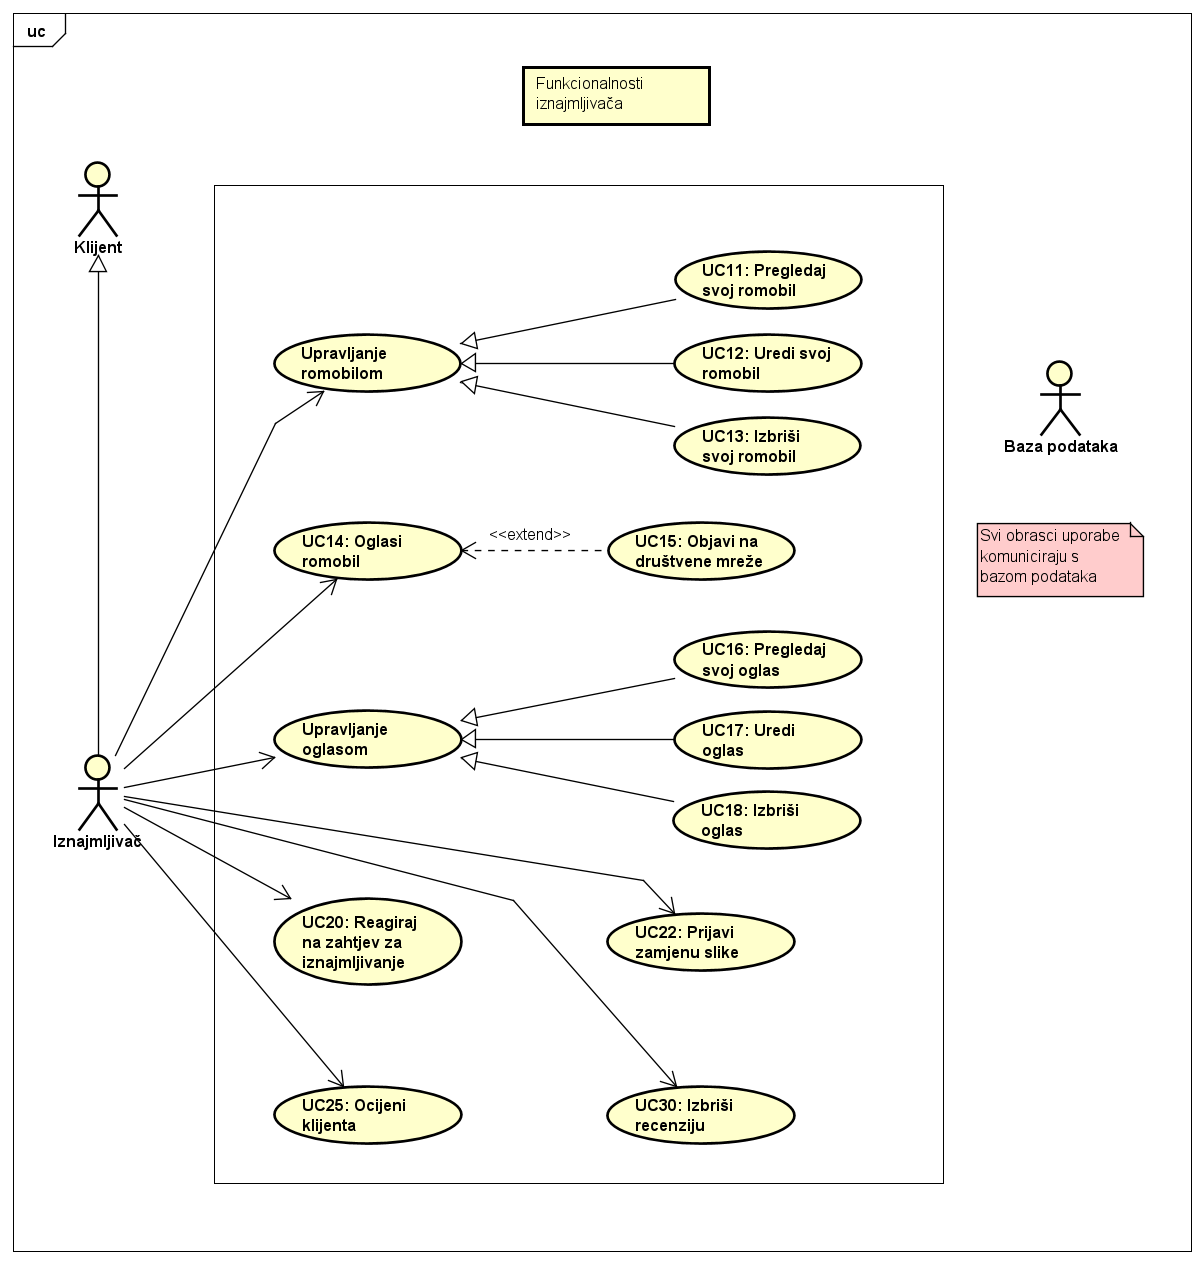
\includegraphics[width=1\linewidth]{dijagrami/iznajmljivac.png}
						\centering
						\caption{Dijagram obrasca uporabe - funkcionalnost iznajmljivača}
						\label{fig:Dijagram obrasca uporabe - funkcionalnost iznajmljivača}
					\end{figure}
					
					\begin{figure} [H]
						
						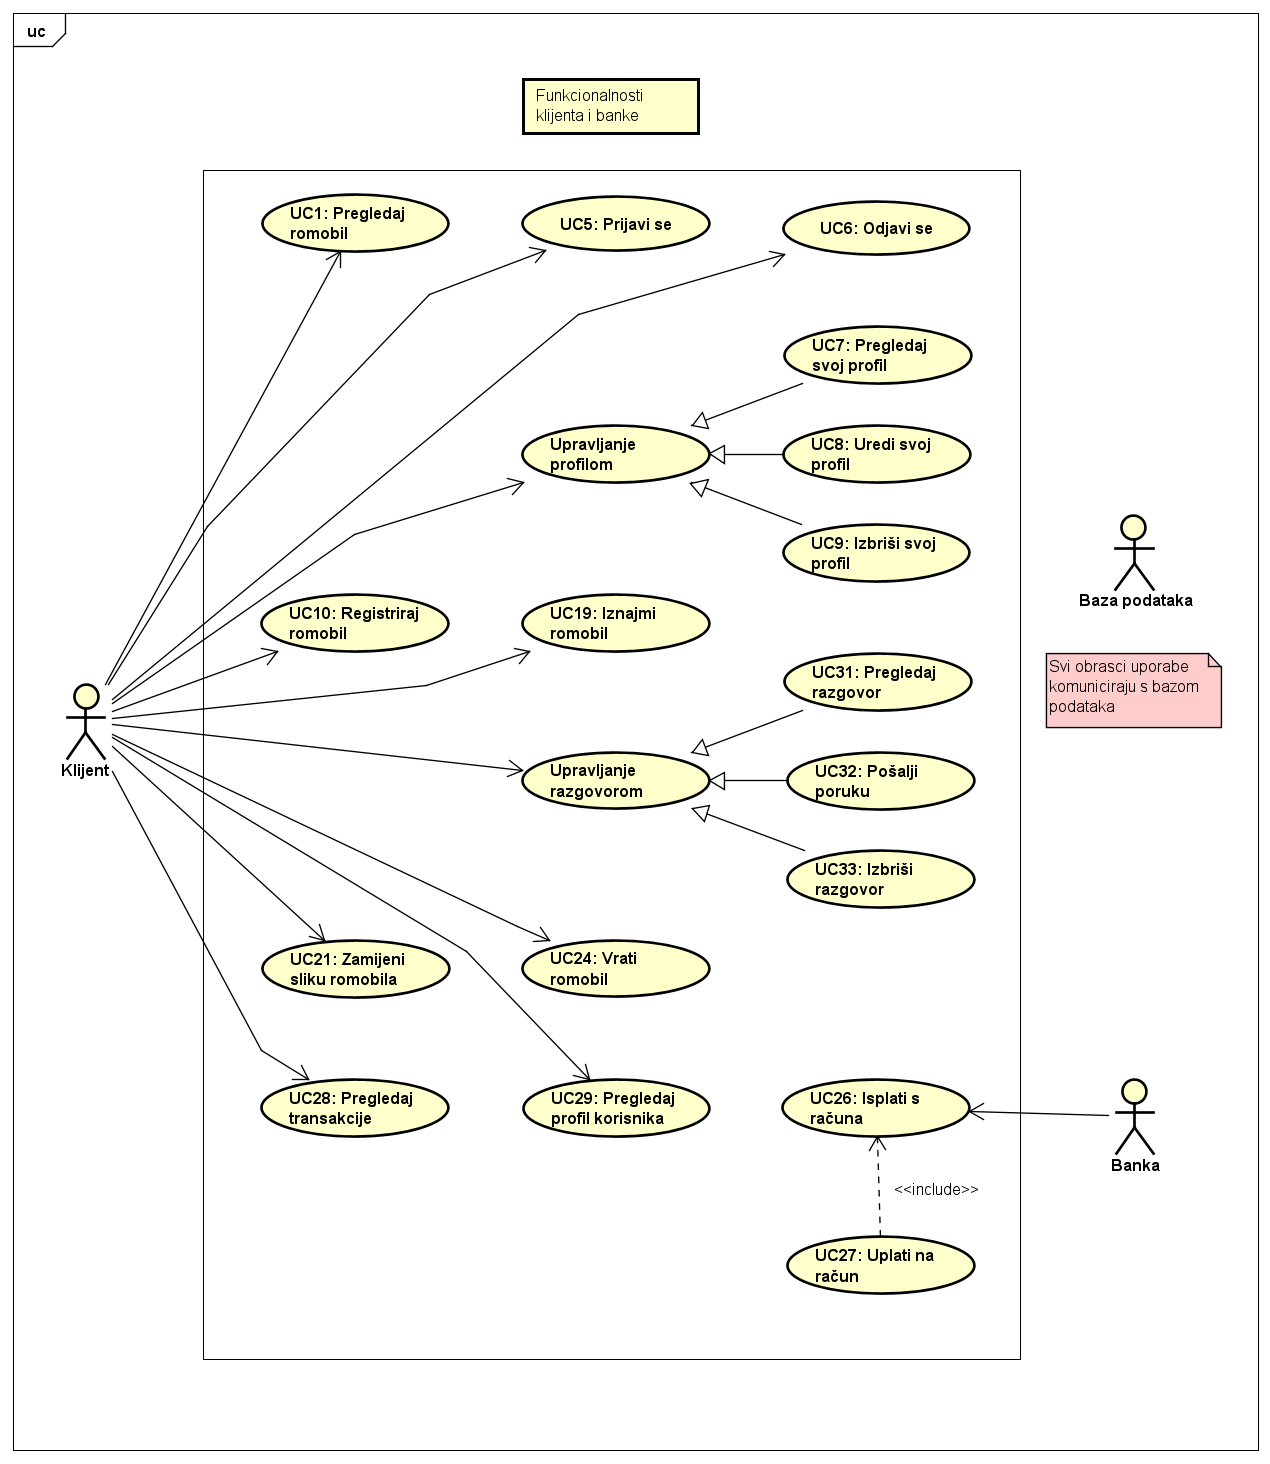
\includegraphics[width=1\linewidth]{dijagrami/klijent_i_banka.png}
						\centering
						\caption{Dijagram obrasca uporabe - funkcionalnost klijenta i banke}
						\label{fig:Dijagram obrasca uporabe - funkcionalnost klijenta i banke}
					\end{figure}
					
					\begin{figure} [H]
						
						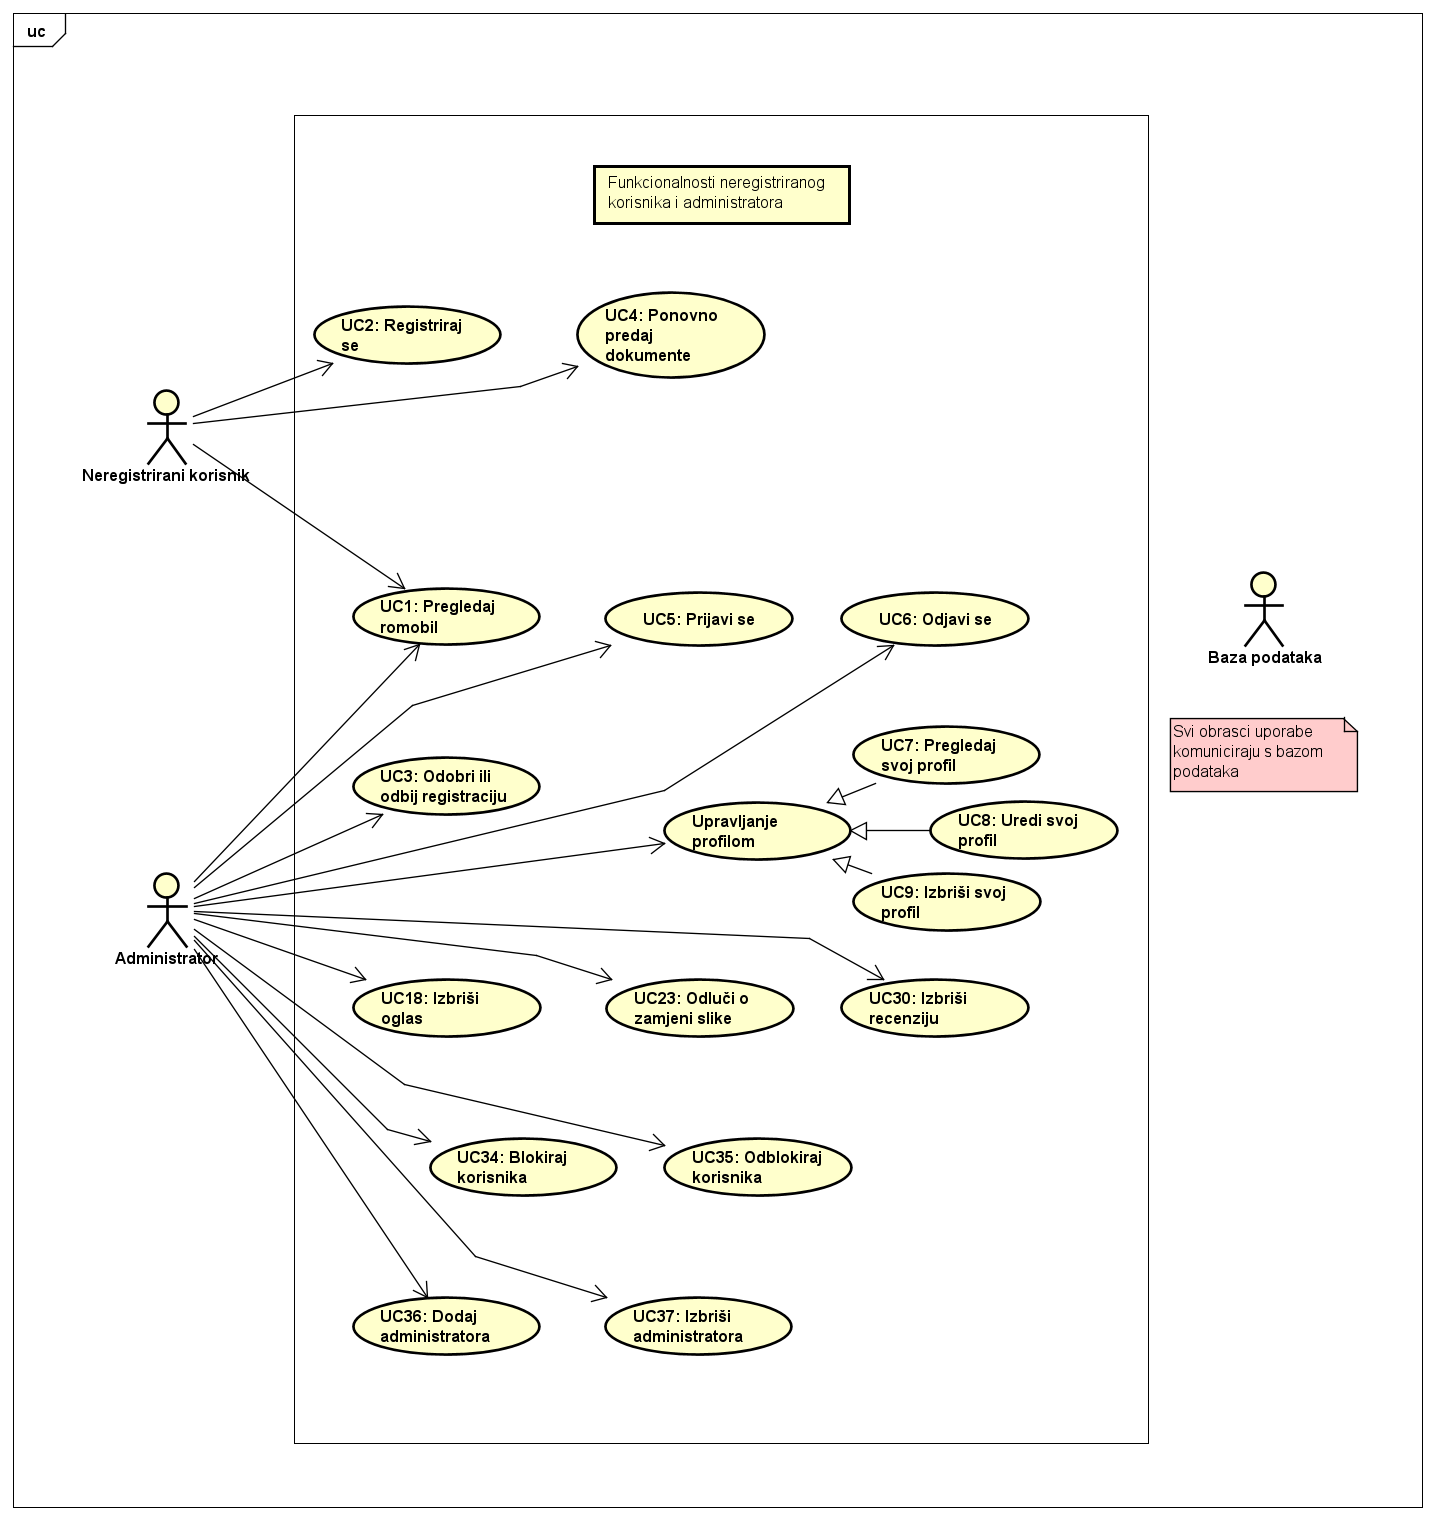
\includegraphics[width=1\linewidth]{dijagrami/neregistrirani_i_admin.png}
						\centering
						\caption{Dijagram obrasca uporabe - funkcionalnost neregistriranog korisnika i administratora}
						\label{fig:Dijagram obrasca uporabe - funkcionalnost neregistriranog korisnika i administratora}
					\end{figure}
					
					
					
				\eject		
				
			\subsection{Sekvencijski dijagrami}

				\subsubsection{Obrazac uporabe UC10 - Registriraj romobil}
						Klijent šalje zahtjev za prikaz stranice s njegovim registriranim romobilima. Poslužitelj iz baze dohvaća registrirane romobile tog klijenta. Ako klijent ima već registrirane romobile, poslužitelj ih prikazuje, inače poslužitelj prikazuje klijentu poruku da nema registriranih romobila. Klijent započinje registraciju romobila tako što zatraži od poslužitelja da mu prikaže obrazac za registraciju. Poslužitelj mu prikazuje prazan obrazac i klijent unosi podatke za registraciju te ih vraća poslužitelju. Poslužitelj provjerava jesu li podatci ispravno uneseni. Sve dok klijent ne unese ispravne podatke ispisuje mu se poruka da su podatci neispravni, unosi nove podatke koje zatim provjerava poslužitelj i vraća informaciju jesu li podatci ispravni ili ne. Kada klijent unese ispravne podatke za registraciju, potvrđuje svoj unos i poslužitelj te podatke prosljeđuje bazi koja pohranjuje registraciju. Romobil se nakon registracije prikazuje među klijentovim registriranim romobilima. Ako klijent do sada nije imao ulogu iznajmljivača, sada mu se dodjeljuje. 
						
						\begin{figure} [H]
							
							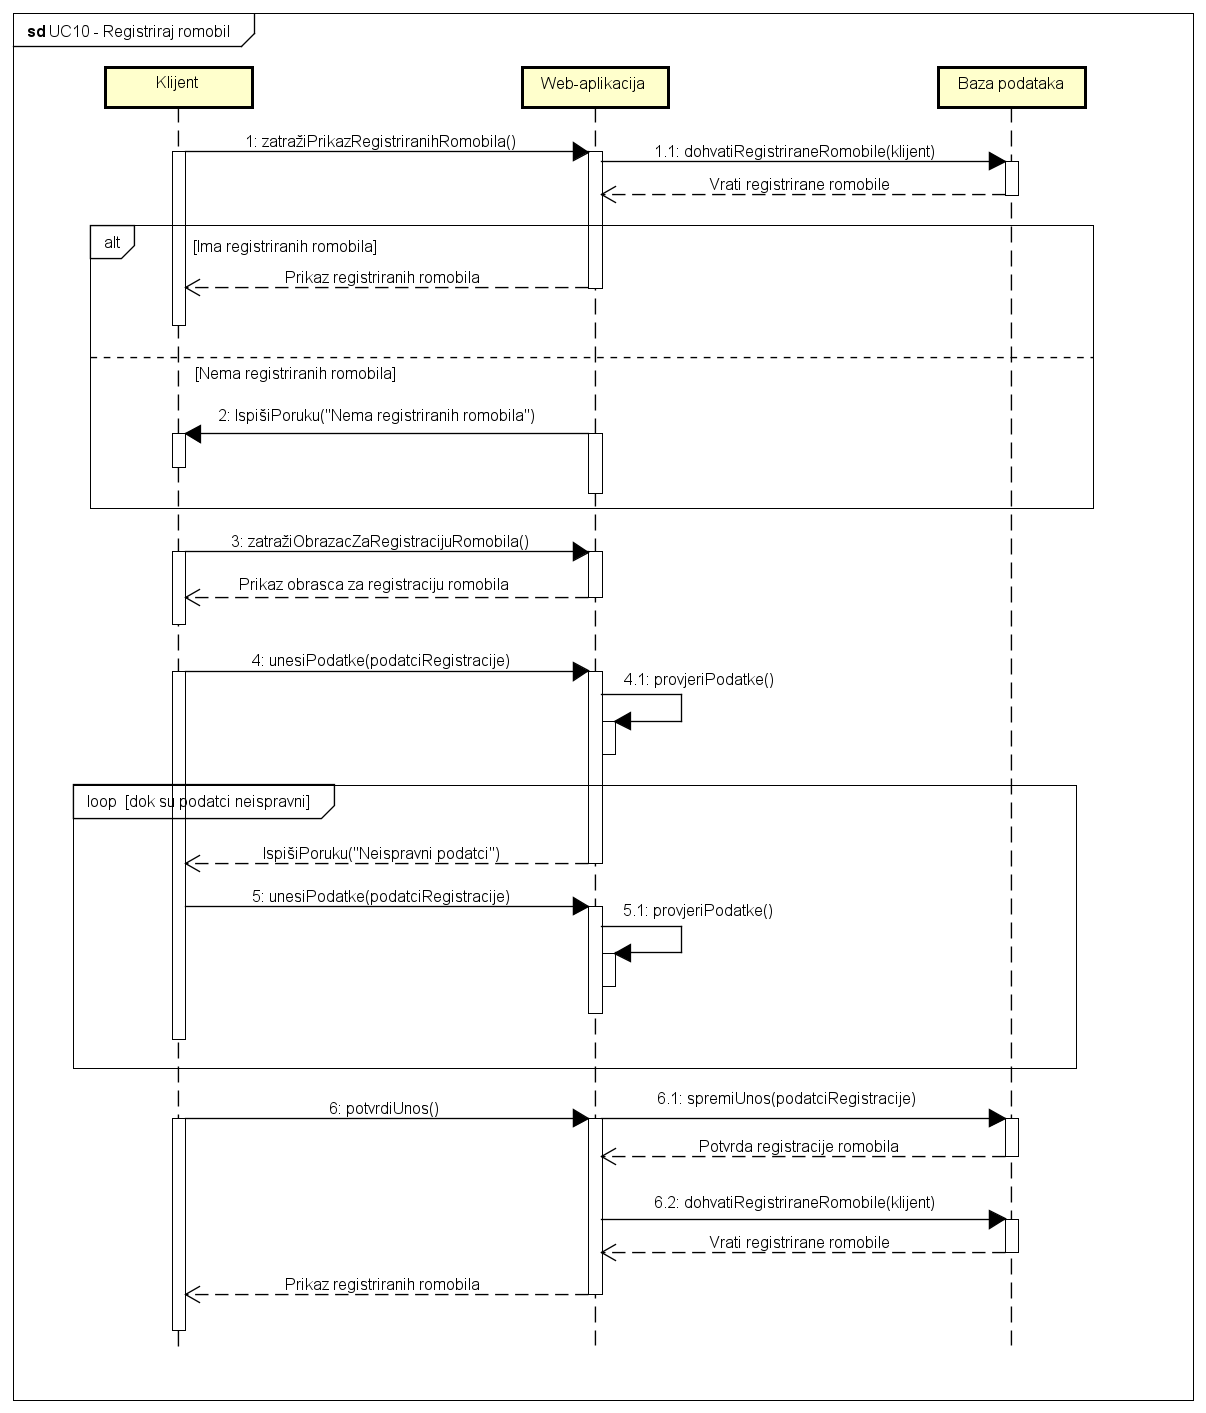
\includegraphics[width=1\linewidth]{dijagrami/UC10 - Registriraj romobil.png}
							\centering
							\caption{Sekvencijski dijagram obrasca UC10 - Registriraj romobil}
							\label{fig:Sekvencijski dijagram obrasca UC10 - Registriraj romobil}
						\end{figure}
				
				\eject

				\subsubsection{Obrazac uporabe UC14 - Oglasi romobil}
						Iznajmljivač šalje zahtjev za prikaz stranice s njegovim registriranim romobilima. Poslužitelj iz baze dohvaća registrirane romobile tog iznajmljivača i prikazuje mu ih. Iznajmljivač započinje stvaranje oglasa tako što zatraži da mu poslužitelj pošalje obrazac koji mora ispuniti. Poslužitelj prikazuje iznajmljivaču obrazac i iznajmljivač unosi podatke o oglasu te ih vraća poslužitelju. Poslužitelj provjerava jesu li podatci ispravno uneseni. Sve dok iznajmljivač ne unese ispravne podatke ispisuje mu se poruka da su podatci neispravni, unosi nove podatke koje zatim provjerava poslužitelj i vraća informaciju jesu li podatci ispravni ili ne. Kada iznajmljivač unese ispravne podatke za registraciju, potvrđuje svoj unos i poslužitelj te podatke prosljeđuje bazi koja pohranjuje oglas. Iznajmljivač dobiva poruku da je oglas uspješno postavljen. Oglas se prikazuje među oglasima dostupnim za iznajmljivanje.
						
						\begin{figure} [H]
							
							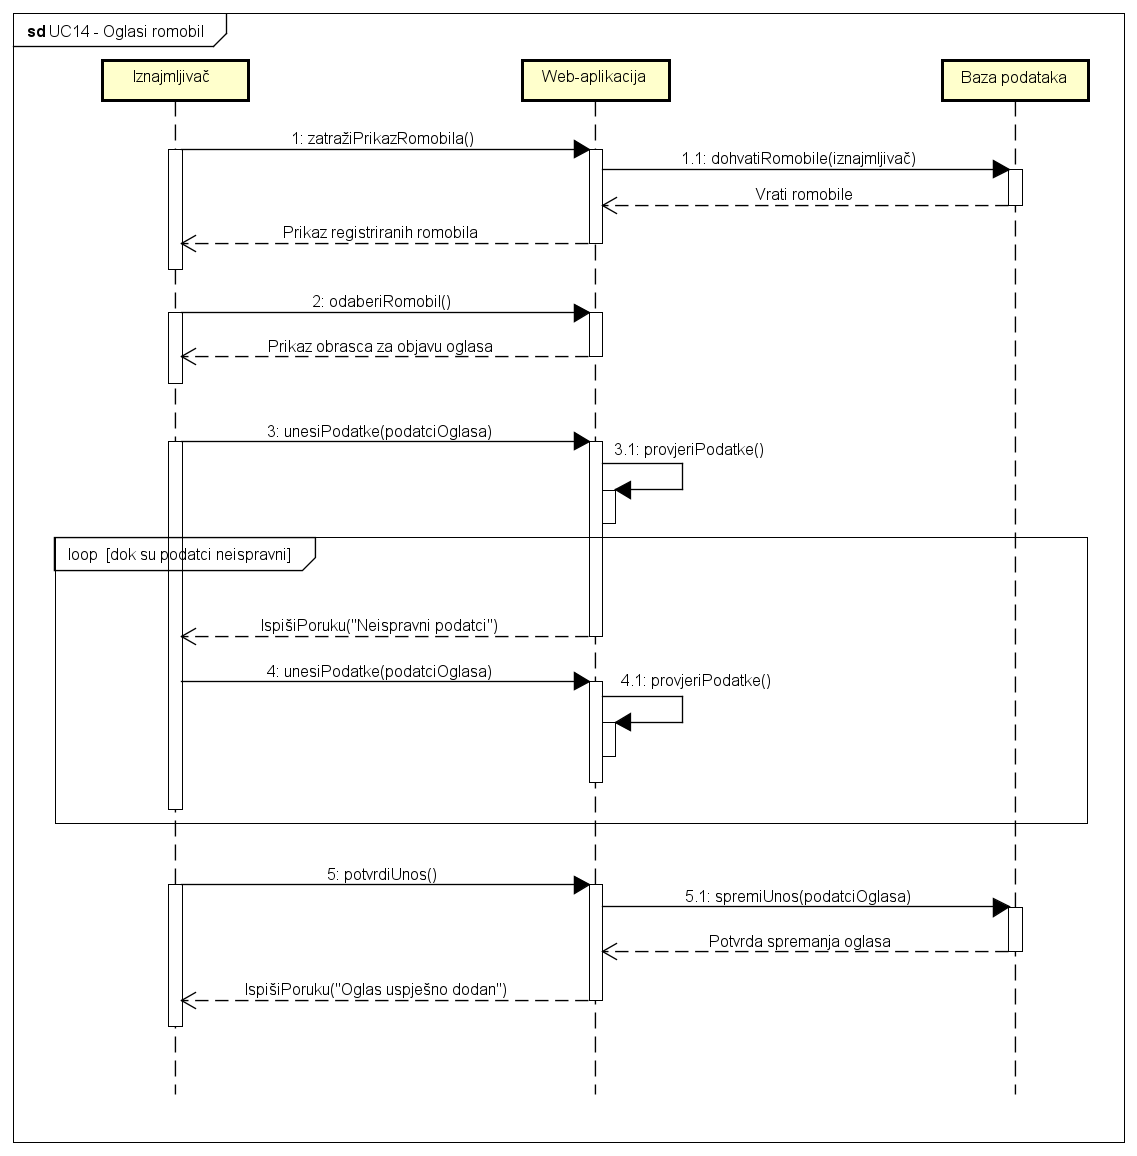
\includegraphics[width=1\linewidth]{dijagrami/UC14 - Oglasi romobil.png}
							\centering
							\caption{Sekvencijski dijagram obrasca UC14 - Oglasi romobil}
							\label{fig:Sekvencijski dijagram obrasca UC14 - Oglasi romobil}
						\end{figure}
						
				\eject

				\subsubsection{Obrazac uporabe UC20 - Reagiraj na zahtjev za iznajmljivanje}
				Iznajmljivač inicira zahtjev za pregled trenutačnih zahtjeva za najam kako bi odgovorio na klijentovu želju za najmom romobila. Poslužitelj preuzima trenutne zahtjeve koje je iznajmljivač poslao i prikazuje ih. Iznajmljivač zatim donosi odluku o prihvaćanju ili odbijanju zahtjeva, a svoj odabir označava u aplikaciji. Poslužitelj prosljeđuje tu informaciju bazi podataka kako bi se ažurirao status zahtjeva. U slučaju prihvaćanja zahtjeva za najam, oglas za najam romobila se uklanja iz baze podataka, a informacija o nedostupnosti romobila se pohranjuje. Nakon što se promjene spreme u bazu podataka, sustav obavještava klijenta o odluci iznajmljivača putem aplikacijske obavijesti.
				
				\begin{figure} [H]
					
					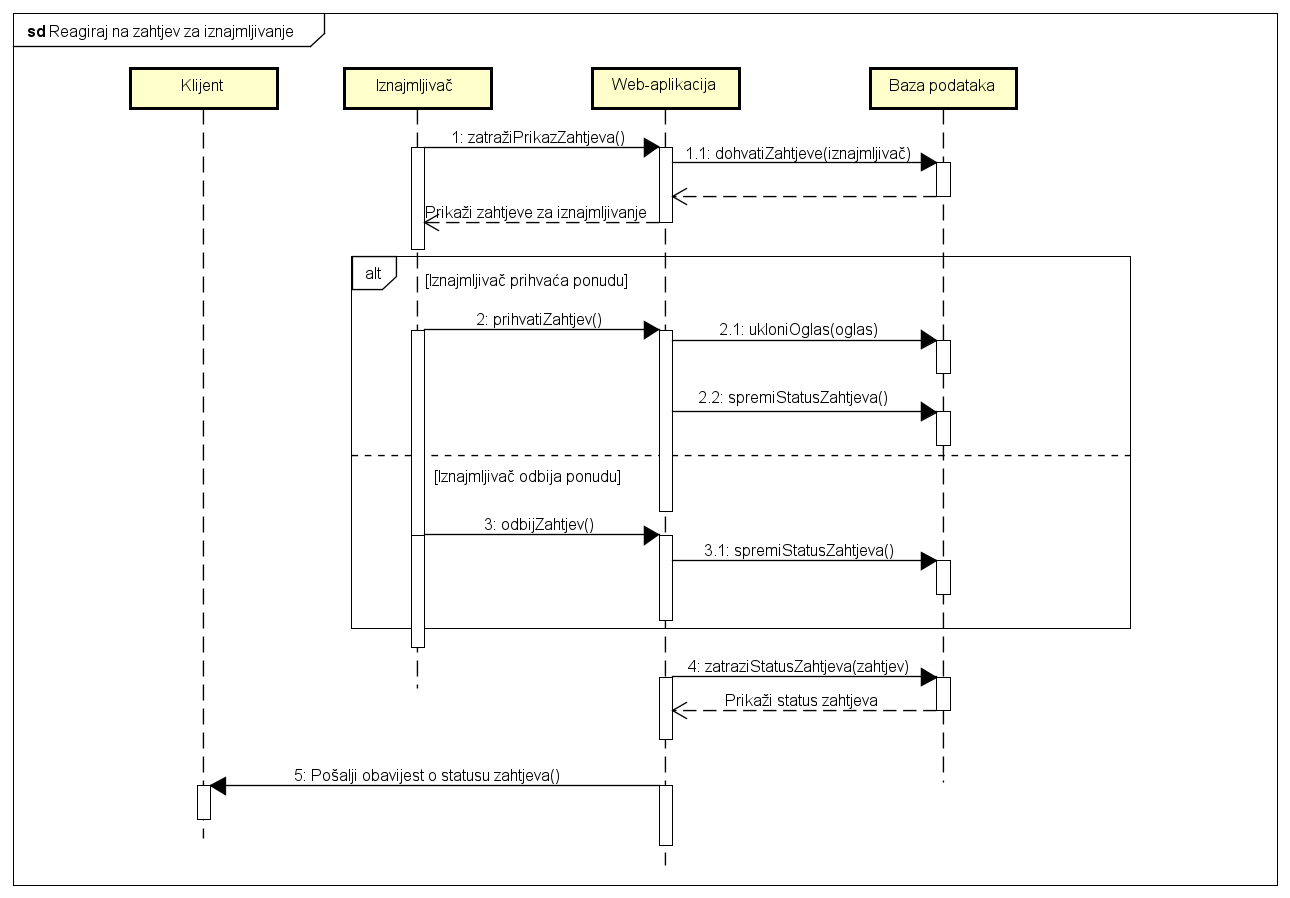
\includegraphics[width=1\linewidth]{dijagrami/UC20 - Reagiraj na zahtjev za iznajmljivanje.png}
					\centering
					\caption{Sekvencijski dijagram obrasca UC20 - Reagiraj na zahtjev za iznajmljivanje}
					\label{fig:Sekvencijski dijagram obrasca UC20 - Reagiraj na zahtjev za iznajmljivanje}
				\end{figure}
				
				\eject

				\subsubsection{Obrazac uporabe UC24 - Vrati romobil}
						Pri povratku romobila na kraju iznajmljivanja klijent zatraži od poslužitelja sve svoje aktivne najmove. Baza podataka pronalazi aktivne najmove tog klijenta i vraća ih poslužitelju. Ako klijent nema nijedan aktivan najam poslužitelj mu vraća poruku koja ga o tome obavještava. U slučaju da aktivni najmovi postoje, poslužitelj ih vraća klijentu. Klijent odabire za koji romobil želi potvrditi da je vraćen i šalje poslužitelju zahtjev da završi iznajmljivanje. Poslužitelj zabilježava kraj u bazi podataka i izračunava broj prijeđenih kilometara i cijenu najma. Informacije o transakciji za taj najam spremaju se u bazu podataka. Poslužitelj prikazujje obavijest o cijeni najma iznajmljivaču i klijentu koji su u najmu sudjelovali.
						
						\begin{figure} [H]
							
							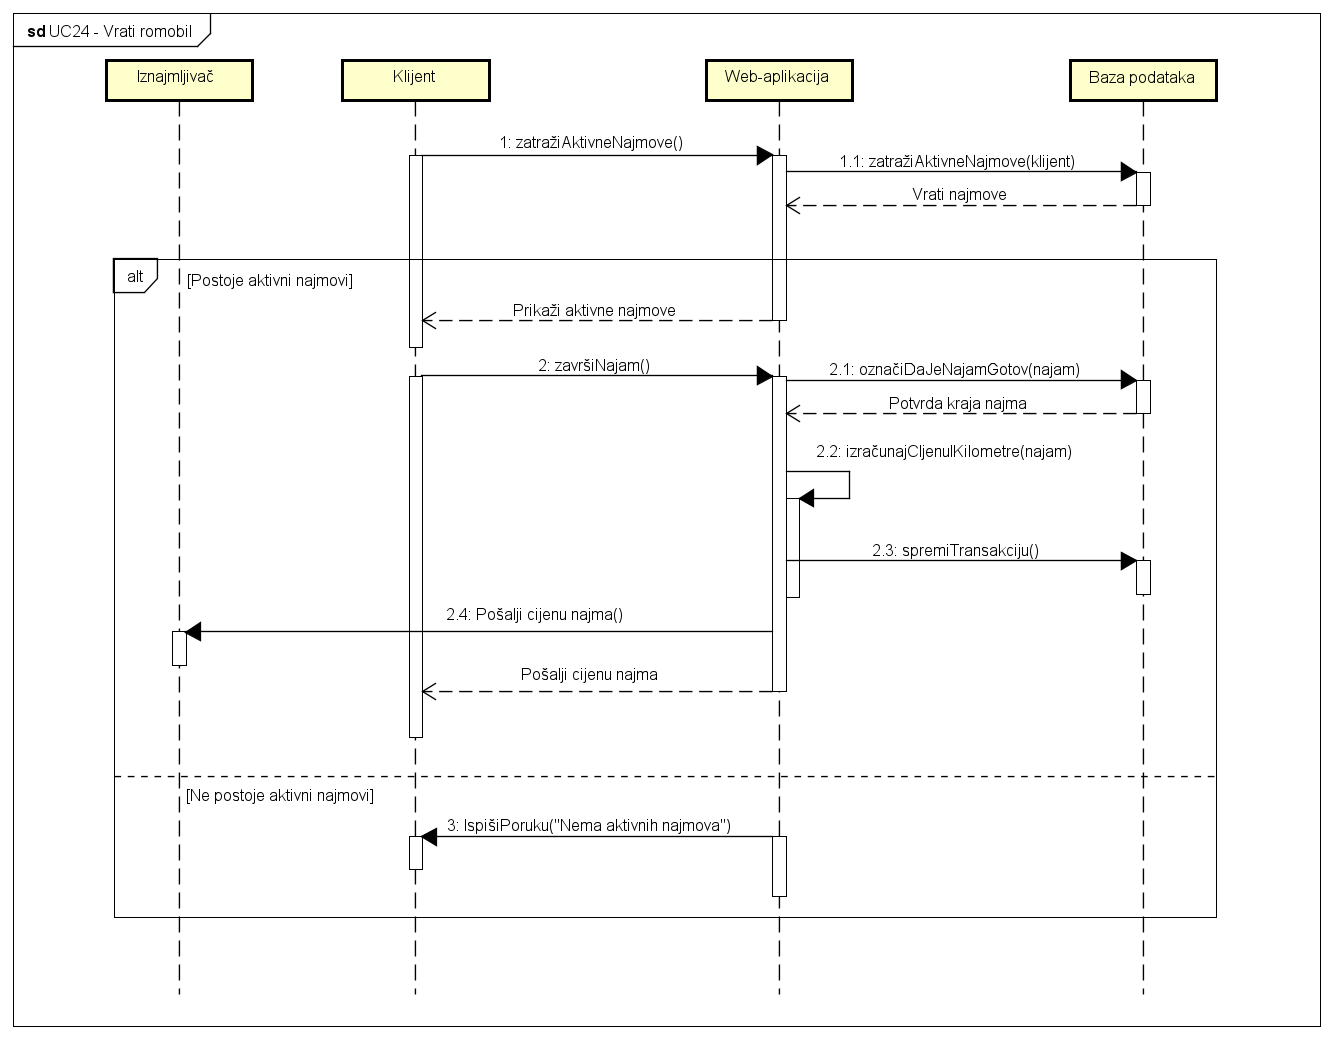
\includegraphics[width=1\linewidth]{dijagrami/UC24 - Vrati romobil.png}
							\centering
							\caption{Sekvencijski dijagram obrasca UC24 - Vrati romobil}
							\label{fig:Sekvencijski dijagram obrasca UC24 - Vrati romobil}
						\end{figure}
				\eject
	

		\section{Ostali zahtjevi}
		
			
		 
			 \begin{packed_item}
			 	\item Aplikacija mora se moći pokrenuti na svakome web-pregledniku
			 	\item Aplikacija mora biti javno dostupna
			 	\item Sustav mora omogućiti rad više korisnika u stvarnom vremenu
			 	\item Korisničko sučelje i sustav moraju podržavati hrvatsku abecedu (dijakritičke znakove)
			 	\item Neispravno korištenje korisničkog sučelja ne smije narušiti funkcionalnost i rad sustava
			 	\item Službena valuta sustavu je EURO (€)
			 	\item Sustav treba biti jednostavan za korištenje
			 	\item Sustav mora biti ostvaren koristeći objektno orijentirane jezike
			 	
			 	
			 \end{packed_item}
			 
			 
			 
	